
\documentclass{beamer}
\usepackage{pgfpages}

% UNCOMMENT FOR FINAL COMPILATION WITH SPEAKER NOTES

\setbeameroption{show notes on second screen=right} % Both
\setbeamertemplate{note page}{\pagecolor{yellow!5}\insertnote}\usepackage{palatino}


\usepackage{graphicx}
\graphicspath{{images/}}


\author{Sam Barrett, 1803086}
\title{{Master's Project Presentation} \\ \texorpdfstring
        {
\includegraphics[scale=0.1]{uobcrest.jpg}}
    }
\institute{{University of Birmingham}}
\date{\today}

\begin{document}

\begin{frame}
\titlepage
\end{frame}


\section{My Topic}
\begin{frame}{My Topic}
    \note{

        \begin{itemize}
            \item I am choosing to focus on the applications of Genetic Algorithms on Theoretical Fully autonomous road networks, with a view to extend into the possible applications of quantum computers on the field in the future. 
            \item  I feel the advent of fully autonomous road networks is a logical next step in making roads safer and more efficient through the use of technology.
            \item Fully autonomous driving trials have been legal in parts of the states for years with the UK following soon.
            \item Most research and all currently implemented systems focus on semi-autonomous environments whereby self-driving vehicles and humans co-exist on shared roads. 
            \item I propose it is both safer, easier and more efficient to implement, fully autonomous road networks where humans are not able to operate their vehicles.
            \item In such a system, sensor data would be shared between all vehicles near instantaneously allowing for much faster and less-selfish route planning, leading to net decreases in travel time. 

        \end{itemize}
    }
    \framesubtitle{Applications of Genetic Algorithms on Fully Autonomous Road Networks}

    \begin{itemize}

        \item Semi-autonomous vehicles are becoming more prevalent 
        \item Roads are becoming more congested with a 78\% increase in motor traffic since 1993 \cite{HighwaysEnglandNetwork2015}
        \item Fully autonomous vehicle trials have been legal in parts of the US since 2015\cite{AutonomousVehiclesSelfDriving}, with the UK set to follow by next year (2021)\cite{UKWantsFully2019}
        \item Much of the current research into autonomous vehicle routing focuses on environments where human drivers are still present
        \item By removing the human element and working on theoretical \textit{fully autonomous road networks} we can make many useful assumptions about the behaviour of other vehicles
        \item The solution to road congestion is not to build bigger roads, it is to optimise the traffic flows.
        \item Just 78.2\% of journeys on the UK Highway Agencies roads were \textit{on time} in the year ending June 2014 \cite{measures02079443095ReliabilityJourneysHighways}

    \end{itemize}
\end{frame}


\section{Literature}
\begin{frame}[allowframebreaks]

    \note{

        \begin{itemize}
            \item As previously mentioned most current research into GA applications within the car industry has a very broad scope. 
            \item Designing possible solutions that would fit into the current road networks easily. 
            \item I am intending to focus on a much more aspirational system, specifically looking at theoretical autonomous Motorways. 
            \item This enables me to overhaul the current road layout which was designed to aid human drivers not the overall efficiency of the system.
        \end{itemize}
        I have chosen to focus on GAs as opposed to other possible AI veins for a few reasons. 
        \begin{itemize}
            \item One personal reason is that I find them particularly interesting. 
            \item One more concrete reason is that they have the very useful property of being both probabilistically optimal and probabilistically complete. Meaning that given infinite time they not only will find \textit{a} solution but they will find \textbf{the} optimal solution. 
            \item And finally they have seen relatively minimal research in the field of vehicle planning with the limelight being taken by technologies such as Deep Learning or Reinforcement Learning
        \end{itemize}


    }

    \frametitle{Literature Review}
    I am currently intending to pursue my research assuming the absence of classical speed lanes as described by Kala and Warwick in \cite{kalaMotionPlanningAutonomous2013}. 

    I have chosen to focus on the applications of Genetic Algorithms on the field for 3 reasons: 
    \begin{enumerate}
        \item It is a class of optimisation algorithms that I find particularly interesting

        \item GAs are \textit{probabilistically optimal and complete}, i.e given infinite time, they will always produce the global optimal solution if such a solution exists

        \item It is a class of algorithm that has seen relatively minimal research in my the specific sub-area 
    \end{enumerate}
\end{frame}

\begin{frame}{Literature Review II}

    \note{
        \begin{itemize}
            \item A many of the technologies being researched with regards to vehicular planning suffer from the same problem from my point of view, they are \textit{black box approaches} meaning given a model, it is very difficult, if not impossible, to reason about and predict the decisions it makes. Such systems could end up making decisions based on imperfections in the training set. Such issues will make these systems less dependable and make people less likely to put their faith in them.
            \item In a paper from 2013, Kala and Warwick proposed a method of representing roads as a set of boundary functions in Cartesian space. All points on the road are defined using these functions as a new basis, this seems to be a good approach as it eliminates the possibility of plotting routes outside of the road space.
        \end{itemize}


    }


    \begin{itemize}
        \item Other approaches involve \textit{black box approaches}. 
        \item The downside of such an approach is that it is very difficult to reason and predict the actions of the system. The ability to assure safety of such a critical system is very important and so GAs offer a much more predictable result
        \item Kala and Warwick \cite{kalaMotionPlanningAutonomous2013} proposed a system of two coordinate systems to safely represent points on the road within Cartesian space.
    \end{itemize}
\end{frame}


\section{Methods}
\begin{frame}
    \frametitle{Methods}
\note{    Talk about what criteria an implementation would need to satisfy, talk about methods to satisfy them and condense lang choice to focus on fulfillment of criteria}
    \framesubtitle{Language Choice} 
    Not final but preliminary implementations have used Julia\cite{JuliaProgrammingLanguage}
    \begin{itemize}
        \item C-like performance
        \item Python \& Matlab -like syntax
        \item Matlab like matrices 
        \item Allows for both OO and functional approaches to problems
        \item Can be compiled
        \item Allows for use of Unicode in variable \& function names so implementations of advanced mathematical expressions are much more readable
    \end{itemize}
\end{frame}

\begin{frame}
    \begin{figure}[Example Julia code]
        \centering
        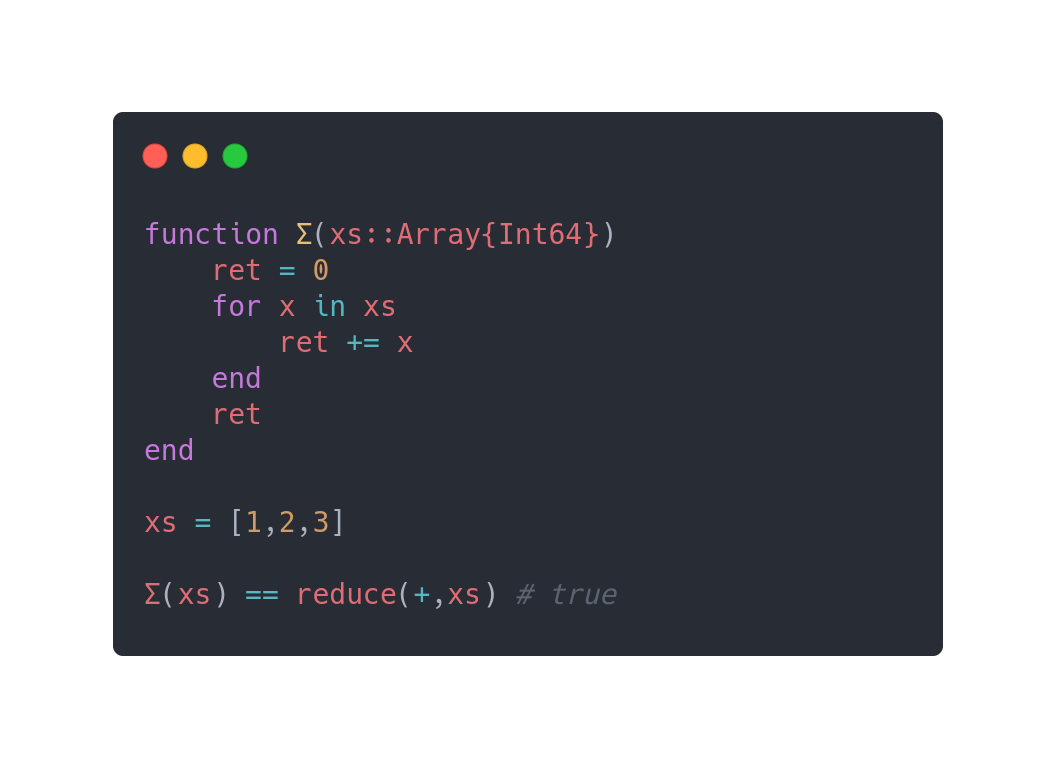
\includegraphics[scale=0.26]{juliaeg.png}
        \caption{Example Julia code}%
        \label{fig:name}
    \end{figure}
\end{frame}

\begin{frame}
Alternative languages include C, Python and Rust
\pause

\textbf{ C:}
\begin{itemize}
    \item Compiles down to binary
    \item Antiquated syntax
    \item Possible (and easy) to write memory unsafe code
    \item Vast array of libraries due to age \& use
    \item No functional properties, harder to implement readable mathematics
\end{itemize}
\pause
\textbf{Python:}
\begin{itemize}
    \item Simple syntax
    \item Wealth of stress-tested libraries
    \item Slow relative to alternatives
    \item unable to compile to binary format
    \item Has some functional capabilities
    \item Has some static typing ability
\end{itemize}
\pause
\end{frame}
\begin{frame}
\textbf{Rust:}
\begin{itemize}
    \item Slower to prototype in as stricter type system to guarantee memory safety
    \item Memory safe, advantage over C/C++
    \item Very performant, runs well on embedded systems
    \item Relatively large binaries due to static dependency linking
    \item Easier to package \& deploy than Julia
\end{itemize}
\end{frame}

\section{Bibliography}
\begin{frame}[allowframebreaks]
\frametitle{References}
\bibliographystyle{abbrv}
\bibliography{lib}
\end{frame}

\end{document}
